\documentclass[tikz]{beamer}
\setbeamercovered{transparent}

\usetheme[bgphoto]{polimi}
% Usage instructions can be found at: https://github.com/elauksap/beamerthemepolimi

\usepackage[utf8]{inputenc}
\usepackage{dsfont}
\usepackage{mwe}
\usepackage{amsmath}
\usepackage[ruled,vlined,linesnumbered]{algorithm2e}
\usepackage{graphicx}
\usepackage{mathtools}
\usepackage{pgfplots}


\usetikzlibrary{positioning}

\title{Protecting HQC against differential\\ power analysis attacks\\}
\subtitle{Cryptography and Architectures for Computer Security project}
\author{Domenico Cacace}
\date{\today}


\begin{document}

\begin{frame}
    \maketitle
\end{frame}

\section{Introduction}
\begin{frame}
    \sectionpage
\end{frame}

\begin{frame}{Quantum Computing 101}
    \begin{block}{What is a quantum computer?}
        A device that performs computations by exploiting the properties of quantum states:
        \begin{itemize}
            \item \textbf{Superposition}: the combination of quantum states is a quantum state
            \item \textbf{Entanglement}: the quantum state of a particle depends on the state of other particles
            %\item \textbf{Interference}
        \end{itemize}
    \end{block}
\end{frame}

\begin{frame}{Quantum Computing 101}
    \begin{columns}[t, totalwidth=1.02\textwidth]
        \begin{column}{0.45\linewidth}
            \begin{block}{What is a qubit?}
                    \begin{itemize}
                        \item The basic unit of quantum information
                        \item Represented as a quantum superposition of two basis states
                    \end{itemize}
                    \begin{equation*}
                        |\psi \rangle = \alpha | 0 \rangle + \beta | 1 \rangle
                    \end{equation*}
            \end{block} 
        \end{column}
        \begin{column}{0.45\linewidth}
            \begin{figure}
                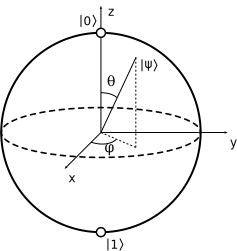
\includegraphics[scale=0.4]{images/Bloch_sphere.png}
            \end{figure}
        \end{column}
    \end{columns}
\end{frame}

\begin{frame}{Classic computers \textit{vs} classic cryptography}
    \begin{block}{Symmetric cryptosystems}
        \textbf{Key enumeration}: perform an exhaustive search on the whole keyspace, $\mathcal{O}(n)$ time
    \end{block}
    \begin{block}{Asymmetric cryptosystems}
        \textbf{General number field sieve}: factor a composite number $n$ is $\mathcal{O}(e^{1.9(\log{n})^{1/3})(\log{\log{n}})^{2/3}})$ (subexponential) time
    \end{block}
\end{frame}

\begin{frame}{Quantum computers \textit{vs} classic cryptography}
    \begin{block}{Symmetric cryptosystems}
        \textbf{Grover's algorithm}: search in a database of $n$ elements in $\mathcal{O}(n^{1/2})$ time and $\mathcal{O}(\log n)$ space
    \end{block}
    \begin{block}{Asymmetric cryptosystems}
        \textbf{Shor's algorithm}: factor a composite number $n$, on a quantum computer, in $\mathcal{O}((\log{n})^2(\log{\log{n}})(\log{\log{\log{n}}}))$ (polynomial) time
    \end{block}
\end{frame}

\begin{frame}{NIST Post-Quantum Cryptography Standardization}
    \begin{block}{Timeline}
        \begin{itemize}
            \item 26/02/16: Announcement of NIST's call for submissions
            \item 21/12/17: Announcement of the first round candidates (69)
            \item 30/01/19: Announcement of the second round candidates (26)
            \item 22/07/20: Announcement of the third round candidates\\ (7 finalists, 8 alternatives)
            \item 2022-2024: Publication of the standard drafts
        \end{itemize}
    \end{block}
\end{frame}

\begin{frame}{NIST Post-Quantum Cryptography Standardization}
    \begin{block}{\textit{Classes} of cryptosystems}
        \begin{itemize}
            \item \textbf{Lattice}: KYBER, FrodoKEM, NTRU Prime, SABER, ...
            \item \textbf{Code-based}: BIKE, Classic McElliece, HQC, LEDAcrypt, ...
            \item \textbf{Supersingular elliptic curve isogeny}: SIKE
            \item \textbf{Mutivariate}: CFPKM, Giophantus
        \end{itemize}
    \end{block}
    We now focus on code-based cryptosystems.
\end{frame}

\section{Coding Theory 101}
\begin{frame}
    \sectionpage
\end{frame}

\begin{frame}{Linear codes}
    Let $\mathcal{V}$ be a vector space of dimension $n$ over $\mathds{F}_2$.
    \begin{block}{Linear codes}
        A \textbf{linear code} $\mathcal{C}$ of length $n$ and dimension $k$ is a
        vector subspace of $\mathcal{V}$ of size $k$ (such a code is also denoted by $[n, k]$).\\
        Elements of $\mathcal{C}$ are called \textbf{codewords}.
    \end{block}
\end{frame}

\begin{frame}{Generating the code}
    Let $\mathcal{C}$ be a $[n, k]$ linear code.
    \begin{block}{Generator Matrix}
         A \textbf{generator matrix} of $\mathcal{C}$ is ${\mathbf{G} \in \mathds{F}_{2}^{k\times n}}$ if
        \begin{equation*}
            \mathcal{C} = \lbrace \mathbf{mG} ~,~ \mathbf{m} \in \mathds{F}_{2}^{k} \rbrace
        \end{equation*}   
        Codewords are linear combinations of the rows of $\mathbf{G}$, so the rows of the generator matrix form a base of the vector subspace $\mathcal{C}$    
    \end{block}
    \begin{block}{Parity check Matrix}
        A \textbf{parity check matrix} of $\mathcal{C}$ is ${\mathbf{H} \in \mathds{F}_{2}^{(n-k)\times n}}$ if
       \begin{equation*}
           \mathcal{C} = \lbrace \mathbf{v} \in \mathds{F}_2^n ~|~ \mathbf{Hv}^\top = \mathbf{0} \rbrace
       \end{equation*}       
   \end{block}
\end{frame}

\begin{frame}{Dual codes}
    Let $\mathcal{C}$ be a $[n, k]$ code, $\mathbf{G}$ and $\mathbf{H}$ its generator and parity check matrices, and $\mathbf{v}$ a codeword of $\mathcal{C}$
        \begin{block}{Dual code}
            $\mathbf{H}$ is the generator of the dual code $\mathcal{C}^\bot$
            \begin{columns}
                \begin{column}{0.45\linewidth}
                    \begin{equation*}
                        \mathbf{G} = \begin{bmatrix} I_k ~|~ P \end{bmatrix}
                    \end{equation*}
                \end{column}
                \begin{column}{0.45\linewidth}
                    \begin{equation*}
                        \mathbf{H} = \begin{bmatrix} -P^\top ~|~ I_{n-k} \end{bmatrix}
                    \end{equation*}
                \end{column}
            \end{columns}
        \end{block}
        \begin{block}{Syndrome}
            We call \textbf{syndrome} of $\mathbf{v}$ the product $\mathbf{Hv}^\top$. From the definition, we have:
            \begin{equation*}
                \mathbf{v} \in \mathcal{C} \Leftrightarrow \mathbf{Hv}^\top = \mathbf{0}
            \end{equation*}
        \end{block}
\end{frame}

\begin{frame}{Circulant Matrices}
    \begin{block}{Circulant matrix}
        Let $\mathbf{v} \in \mathds{F}_2^p = (v_0, \cdots, v_{p-1})$. The circulant matrix induced by $\mathbf{v}$ is defined as:
        \begin{equation*}
            \mathbf{circ(v)} = \begin{pmatrix}
                v_0 & v_1 & \cdots & v_{p-1} \\
                v_{p-1} & v_0 & \cdots & v_{p-2} \\
                \vdots & \vdots & \ddots & \vdots \\
                v_1 & v_2 & \cdots & v_0
                \end{pmatrix} \in \mathds{F}_2^{p\times p}
        \end{equation*}
        The algebra of $p \times p$ circulant matrices over $\mathds{F}_2$ is isomorphic to the algebra of polynomials in the ring $\mathds{F}_2[x]/(x^p - 1)$\\
        \begin{equation*}
        \mathbf{circ(v)} \simeq v_0 + v_1x^1 + \cdots + v_{p-1}x^{p-1}
        \end{equation*}
    \end{block}
\end{frame}

\begin{frame}{Quasi-cyclic codes}
    \begin{block}{Quasi-cyclic codes}
        A \textbf{quasi-cyclic code} $\mathcal{C}$ is a linear code $[n, k]$, with $n = pn_0$ and $k=pk_0$, such that every cyclic shift of a codeword by $n_0$ symbols yields another codeword
    \end{block}
    \begin{block}{}
        A generator matrix $\mathbf{G}$ of the QC-code $\mathcal{C}$ has the form:
        \begin{equation*}
            \mathbf{G} = 
            \begin{bmatrix}
                C_{1, 1} & C_{1, 2} & \cdots & C_{1, n_0} \\
                C_{2, 1} & C_{2, 2} & \cdots & C_{2, n_0} \\
                \vdots & \vdots & \ddots & \vdots \\
                C_{k_0, 1} & C_{k_0, 2} & \cdots & C_{k_0, n_0}
                \end{bmatrix} \in \mathds{F}_2^{k \times n}
        \end{equation*}
        where each entry $C_{i, j}$ is a $p \times p$ circulant matrix.
    \end{block}
\end{frame}

\begin{frame}{Metrics}
    Let $\mathcal{C}$ be a $[n, k]$ code, and $\mathbf{v, w}$ codewords of $\mathcal{C}$
    \begin{block}{Hamming distance}
        The \textbf{Hamming distance} between two vectors is the Hamming weight of the difference of the vectors
        \begin{equation*}
            d(\mathbf{v, w}) = \mathtt{wt}(\mathbf{v - w})
        \end{equation*}
    \end{block}
    \begin{block}{Minimum distance}
        The \textbf{minimum distance} of a code is the minimum distance among any couple of codewords
        \begin{equation*}
            d_{min} = \min_{\mathbf{v, w} \in \mathcal{C}, \mathbf{v \neq w}} \mathtt{wt}(\mathbf{v-w})
        \end{equation*}
    \end{block}
\end{frame}

\begin{frame}{Decoding a code}
    \begin{block}{Transmission errors}
        When travelling on a channel, the original codeword $\mathbf{x}$ might be corrupted, so that the received codeword is 
        \begin{equation*}
            \mathbf{y} = \mathbf{x} + \mathbf{e} \text{, with } \mathbf{e} \text{ error vector}
        \end{equation*}
        For $\mathtt{wt}(\mathbf{e}) \leq \delta = \lfloor \frac{d_{min} - 1}{2} \rfloor$ we are able to recover the original codeword
    \end{block}
\end{frame}

\begin{frame}{Decoding a code}
    Let $\mathbf{y = x+e}$ be the received codeword
    \begin{block}{Minimum distance decoding}
        Pick a codeword $\mathbf{u}$ that minimizes the Hamming distance $d(\mathbf{u, y})$\
        \begin{equation*}
            \textsf{Decode}(\mathbf{y}) = \arg\min_{\mathbf{u} \in \mathcal{C}} d(\mathbf{u, y})
        \end{equation*}
    \end{block}
    \begin{block}{Syndrome decoding}
        By the definition of syndrome of a codeword we have:
        \begin{equation*}
            \mathbf{Hy} = \mathbf{H(x+e)} = \mathbf{Hx+He} = \mathbf{0 + He} = \mathbf{He} 
        \end{equation*}
    \end{block}
\end{frame}

\begin{frame}{Hard problems of coding theory}
    \begin{block}{Syndrome decoding problem~\cite{berlekamp1978inherent}}
        Given a $[n, k]$ code $\mathcal{C}$ with parity matrix $\mathbf{H}$, the syndrome $\mathbf{y} \in \mathds{F}_2^{n-k}$ and $w \leq n$, find
        the codeword $\mathbf{x} \in \mathds{F}_2^n$ such that $\mathbf{Hx}^\top = \mathbf{y}^\top$ and $\mathtt{wt}(\mathbf{x}) = w$. 
    \end{block}
\end{frame}


\section{Hamming Quasi-Cyclic}
\begin{frame}
    \sectionpage
\end{frame}

\begin{frame}{Overview}
    \begin{block}{HQC}
        One of the third round alternative candidates
        \begin{itemize}
            \item IND-CPA Public Key Encryption
            \item IND-CCA2 Key Encapsulation Mechanism
            \item Based on a variant of the syndrome decoding problem
            \item Employs quasi-cyclic codes to shorten key sizes
        \end{itemize}
    \end{block}
    \begin{block}{Codes}
        HQC employs two codes:
        \begin{itemize}
            \item a decodable$\mathcal{C} [n, k]$ generated by $\mathbf{G}\in \mathds{F}_{2}^{k\times n}$ (public) 
            \item a random $[2n, n]$ code with parity-check matrix $\mathbf{H} = (\mathbf{I}_n | \mathbf{rot(h)})$
        \end{itemize}
    \end{block}
\end{frame}

\begin{frame}{Public Key Encryption}
    \begin{block}{Setup}
        Generate the parameters $(n, k, \delta, w, w_r, w_e)$ for the corresponding security level $\lambda$
    \end{block}
    \begin{block}{Key Generation}
        \begin{itemize}
            \item Generate $seed_h \xleftarrow{\$} \lbrace 0, 1 \rbrace^\lambda$
            \item Generate $\mathbf{h} \xleftarrow{seed_h} \mathds{F}_2^n$ 
            \item Generate $(\mathbf{x, y}) \xleftarrow{\$} \mathds{F}_2^n$, with $\omega(\mathbf{x}) = \omega({\mathbf{y}}) = w$
            \item Calculate $\mathbf{s = x + hy}$
        \end{itemize}
        \begin{columns}
            \begin{column}{0.45\linewidth}
                \begin{center}
                    \textsf{pk} = $(\mathbf{h, s})$
                \end{center}
            \end{column}
            \begin{column}{0.45\linewidth}
                \begin{center}
                    \textsf{sk} = $(\mathbf{x, y})$
                \end{center}
            \end{column}
        \end{columns}
    \end{block}
\end{frame}

\begin{frame}{Public Key Encryption}
    To encrpyt a message $\mathbf{m} \in \mathds{F}_2^k$ :
    \begin{block}{Encryption}
        \begin{itemize}
            \item Generate $(\mathbf{r_1, r_2}) \xleftarrow{\$} \mathds{F}_2^n$, with $\omega(\mathbf{r_1}) = \omega({\mathbf{r_2}}) = w_r$
            \item Generate $\mathbf{e} \xleftarrow{\$} \mathds{F}_2^n$, with $\omega(\mathbf{e}) = w_e$
            \item Calculate $\mathbf{u = r_1 + hr_2}$
            \item Calculate $\mathbf{v = mG +sr_2 + e}$
        \end{itemize}
        \begin{center}
            \textsf{ctx} = $(\mathbf{u, v})$
        \end{center}
    \end{block}
\end{frame}

\begin{frame}{Public Key Encrpytion}
    \begin{block}{Decryption}
        From the \textsf{ctx} = $(\mathbf{u, v})$ and the private key \textsf{pk} = $(\mathbf{x, y})$:
        \begin{equation*}
            \begin{aligned}
                \mathbf{v - u\cdot y} & \mathbf{ = (mG +s\cdot r_2 + e) - (r_1 + h\cdot r_2)y = mG + x\cdot r_2 -r_1\cdot y + e}\\
                &\mathbf{ = mG + (x + h\cdot y)r_2 + e - (r_1\cdot y  + h\cdot r_2\cdot y)}\\
                &\mathbf{ = mG + x\cdot r_2 + h\cdot y\cdot r_2 + e - r_1\cdot y - h\cdot r_2\cdot y}\\
                &\mathbf{ = mG + x_2 - r_1\cdot y + e}\\
            \end{aligned}
        \end{equation*}
        So we have $\mathbf{m} = \mathcal{C}.\textsf{Decode}(\mathbf{v - u\cdot y})$ whenever
        \begin{equation*}
            \omega(\mathbf{x\cdot r_2 - r_1\cdot y + e}) \leq \delta
        \end{equation*}
    \end{block}
\end{frame}

\begin{frame}{Key Encapsulation Mechanism}
    By applying the Fujisaki-Okamoto transformation it is possible to build a IND-CCA2 KEM.
    Let $\mathcal{G, H, K}$ be hash functions and $\mathcal{E}$ an instance of \textsf{HQC.PKE}
    \begin{block}{}
        \begin{itemize}
            \item \textbf{Setup}: generate the parameters $\lambda$ as in \textsf{HQC.PKE}, except that k will be the length of the key to be exchanged
            \item \textbf{KeyGen}: as in \textsf{HQC.PKE}
        \end{itemize}
    \end{block}
\end{frame}

\begin{frame}{Key Encapsulation Mechanism}
    Let $\mathcal{G, H, K}$ be hash functions and $\mathcal{E}$ an instance of \textsf{HQC.PKE}
    \begin{block}{Encapsulation}
        \begin{itemize}
            \item Generate the seed $\mathbf{m} \xleftarrow{\$} \mathds{F}_2^k$ and the randomness $\theta \leftarrow \mathcal{G}(\mathbf{m})$
            \item Generate the ciphertext $\mathbf{c} \leftarrow (\mathbf{u, v}) = \mathcal{E}.\textsf{Encrypt}(\textsf{pk}, \mathbf{m}, \theta)$
            \item Derive the symmetric key $K = \mathcal{K}(\mathbf{m, c})$
            \item Calculate $\mathbf{d} \leftarrow \mathcal{H}(\mathbf{m})$
            \item Send the couple $(\mathbf{c, d})$
        \end{itemize}
    \end{block}
\end{frame}

\begin{frame}{Key Encapsulation Mechanism}
    Let $\mathcal{G, H, K}$ be hash functions and $\mathcal{E}$ an instance of \textsf{HQC.PKE}
    \begin{block}{Decapsulation}
        \begin{itemize}
            \item Decrypt $\mathbf{m}^{'} \leftarrow \mathcal{E}.\textsf{Decrypt}(\textsf{sk}, \mathbf{c})$
            \item Compute $\theta^{'} \leftarrow \mathcal{G}(\mathbf{m}^{'})$ and $\mathbf{c}^{'} \leftarrow \mathcal{E}.\textsf{Encrpyt}(\textsf{pk}, \mathbf{m}^{'}, \theta^{'})$
            \item Check that $\mathbf{c = c^{'}}$ and $\mathbf{d} = \mathcal{H}(\mathbf{m}^{'})$
            \item Derive the shared key $K \leftarrow \mathcal{K}(\mathbf{m, c})$
        \end{itemize}
    \end{block}
\end{frame}

\section{Masking}

\begin{frame}
    \sectionpage
\end{frame}

\begin{frame}{Side Channel Attacks}
    Implementations of theoretically secure cryptosystems may \textit{leak} some information, allowing an 
    attacker to extract secret data.
    \begin{block}{Side Channel Vulnerabilities}
        Side channel attacks take use of different leakage sources, such as:
        \begin{itemize}
            \item Execution time
            \item Power consumption
            \item Electromagnetic radiation
            \item Differential faults
        \end{itemize}
    \end{block}
\end{frame}

\begin{frame}{Power Analysis}
    \begin{block}{Simple Power Analysis}
        Analyze the electrical current drawn by the device over time: different operations may have different power consumption.
    \end{block}
    \begin{block}{Differential Power Analysis}
        Statistically analyze the power consumption of the device over different executions: detect biases between, for example, a known secret key and a unknown one.
    \end{block}
\end{frame}

\begin{frame}{Power Analysis}
    \begin{figure}
        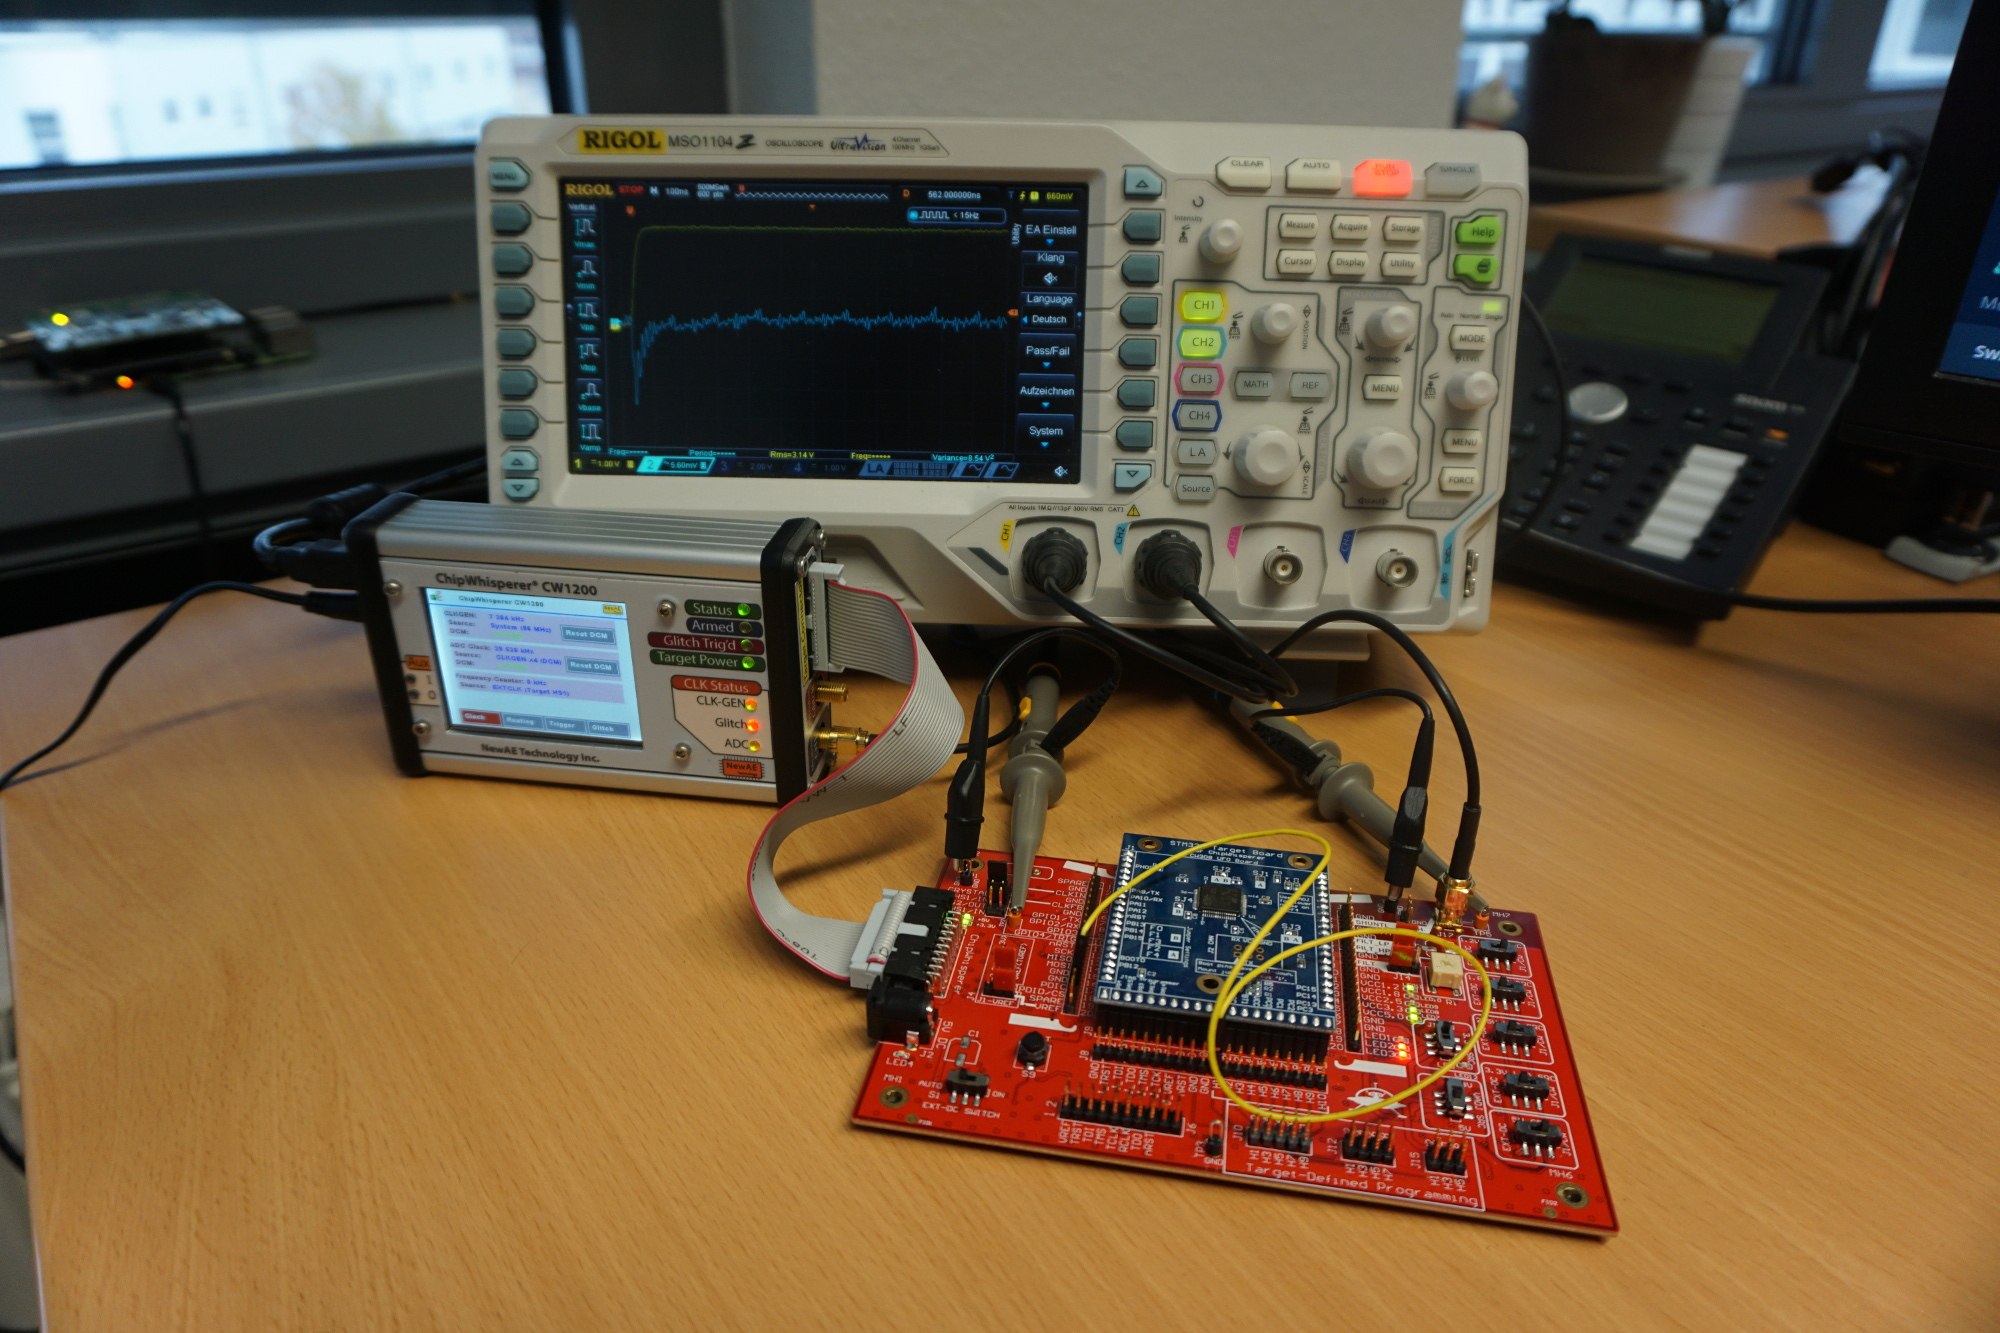
\includegraphics[scale=0.6]{images/chipwhisperer_with_target_and_oscilloscope.jpg}
        \caption{ChipWhisperer}
        % \footnote{https://www.schutzwerk.com/en/43/posts/poweranalysis\_1/}
    \end{figure}
    
\end{frame}

\begin{frame}{Countermeasures to Power Analysis}
    Power analysis attacks are usually passive, so they cannot be detected by the device.
    \begin{block}{}
        To mitigate the effectiveness of these attacks, it is possible to:
        \begin{itemize}
            \item \textbf{SPA}: avoid branches with conditions that depend on secret data
            \item \textbf{DPA}: \textit{mask} the secret data when performing operations on them
        \end{itemize}
    \end{block}
    \begin{block}{Masking}
        Given a secret $x$, we can split it into $d$ \textit{shares} in such a way that
        \begin{equation*}
            x = x_0 \odot x_1 \cdots \odot x_{d-1}
        \end{equation*}
        for some operation $\odot$ (e.g. XOR in binary fields).
    \end{block}
\end{frame}

\begin{frame}{Securing AND gates}
    \begin{block}{Probing Model~\cite{ishai2003private}}
        Given an algorithm that operates on data split among $d$ shares, we say that the algorithm is 
        secure against a $(d-1)$-th order probing attack if, on input $x = (x_1, \cdots, x_d)$, it admits no
        tuple of $d-1$ (or less) shares that depends on $x$
    \end{block}
    \begin{block}{Ishai-Sahai-Wagner’s Scheme}
        Let $x = (x_1, \cdots, x_d), y = (y_1, \cdots, y_d)$ binary variables: to securely compute $x \wedge y$ at order $\lfloor d/2 \rfloor$:
        \begin{itemize}
            \item Pick a random bit $r_{i, j}$
            \item Compute $r_{j, i} = (r_{i, j} + (x_i \wedge y_j)) + (x_j \wedge y_i)$
            \item Compute $c_i = (x_i \wedge y_j) + \sum_{j \neq i} r_{i, j}$ 
        \end{itemize}
    \end{block}
\end{frame}

\begin{frame}{Securing multiplications}
    The ISW scheme can be extended from $\mathds{F}_2$ to $\mathds{F}_2^{n}$, increasing its security to $d$-th order attacks
    \begin{block}{Rivain-Prouff's Scheme}
        Let $a = (a_1, \cdots, a_d), b = (b_1, \cdots, b_d)$, with $ a_i, b_i \in \mathds{F}_2^n$
        \begin{itemize}
            \item Calculate $c_i \leftarrow a_i\cdot b_i$ for each share
        \end{itemize}
        For $i$ from 1 to $d$ and $j$ from $i+1$ to $d$:
        \begin{itemize}
            \item Extract a random value $s \xleftarrow{\$} \mathds{F}_2^n$
            \item Calculate $s^{'} \leftarrow (s + (a_i \cdot b_j)) + (a_j \cdot b_i)$
            \item Calculate $c_i \leftarrow c_i + s$ and  $c_j \leftarrow c_j + s^{'}$ 
        \end{itemize}
        The sum of the shares $(c_1, \cdots, c_d)$ yields the product $a\cdot b$
    \end{block}
\end{frame}
\section{Implementation}
As a starting point, we take the third version of the reference implementation\footnote{\href{https://pqc-hqc.org/download.php?file=hqc-reference-implementation\_2021-06-06.zip}{https://pqc-hqc.org/download.php?file=hqc-reference-implementation\_2021-06-06.zip}}; this is a self-contained C implementation that can be ported on virtually any architecture as-is.

\subsection*{\textbf{Target}}
Our target architecture is \texttt{ARMv7E}: in particular, our tests are run on the STM F401-RE board mounting a Cortex\textsuperscript{\textregistered} M4 processor. This particular board is equipped with 512KB of flash memory and 96KB of RAM: due to this characteristics and the large memory footprint of the cryptosystem, we were able to run HQC only at security level 1 (corresponding to 128 bits of security).
In order to interact with the system we employ the Hardware Abstraction Layer (HAL) drivers, generated by STM32CubeMX specifically for our configuration. We use the drivers to notify when the encryption process is taking place through the LED on the board and to allow communications over the USB debug interface, redirecting in the \texttt{syscalls.c} file the standard output to the debug bridge for logging purposes.
To generate random variables required we employ the \texttt{seedexpander} function from SHAKE256~\cite{dworkin2015sha}.

\subsubsection*{\textbf{Objects representations}}
Elements of the various binary fields are represented as arrays. For randomly generated values, we employ the \texttt{seedexpander} function on a 40B seed.\\
The secret key \textsf{sk} = $(\mathbf{x}, \mathbf{y})$ is generated by $\mathbf{seed1}$, while the parity matrix $\mathbf{h}$ of the public key \textsf{pk}=$(\mathbf{h}, \mathbf{s})$ is generated by $\mathbf{seed2}$; the same principle applies for the random masks employed in the \texttt{safe\_mul} function. These values are sampled uniformly from the respective fields, with a given Hamming weight.\\
In all the multiplications, one of the operands is always a sparse polynomial: these polynomials are represented with a position vector of $\omega$ coordinates, containing the orders of the nonzero coefficients.

\subsubsection*{\textbf{Multiplication and masking}}
The multiplication over $\mathds{F}_2[X]/(X^n-1)$ is implemented with a slight variation of the scoolbook multiplication algorithm, since the sparsity of one of the operands yields a lower computational complexity than other methods.
This approach leaks information about the operands, which should remain secret: to overcome this problem we implemented a first-order masked multiplication scheme.\\

The dense ($a$) and sparse ($b$) polynomials are split in two halves, which are then combined accordingly to the ISW scheme; the \texttt{add} and \texttt{mult} function are an abstraction of the instructions that perform the addition and multiplication.

\begin{algorithm}
    \SetAlgoLined
    \SetKwFunction{secure_mult}{secure_mult}
    \KwIn{$a = (a_0a_1) \in \mathds{F}_2^n$ dense polynomial, $b = (b_0b_1)$ sparse polynomial, $\omega(b) = w$}
    \KwOut{$res, mask$ such that $res\oplus mask = a\cdot b$}
    \KwData{$temp_1, temp_2 \in \mathds{F}_2^n$}
    \SetKwProg{Fn}{function}{:}{}
    \BlankLine
    \BlankLine

    $mask \xleftarrow{\mathdollar_w} \mathds{F}_2^n$\\

    $temp_1 \leftarrow \texttt{mult}(a_1, b_0)$\\
    $temp_2 \leftarrow \texttt{mult}(a_0, b_1$)\\

    $res \leftarrow \texttt{add}(mask, temp_1)$\\
    $res \leftarrow \texttt{add}(res, temp_2)$\\

    $temp_1 \leftarrow \texttt{mult}(a_1, b_1)$\\
    $temp_2 \leftarrow \texttt{mult}(a_0, b_0$)\\

    $res \leftarrow \texttt{add}(res, temp_2)$\\
    $mask \leftarrow \texttt{add}(mask, temp_1)$\\

    \Return$res$, $mask$    
    \caption{First-order masked multiplication, 2 shares}
\end{algorithm}

We then generalized the masking procedure any number of by creating a small code generator to unroll the loops and reduce the execution time. 
We implemented and tested the masking procedure for $d \in \lbrace 2, 3, 4\rbrace$, as the number of operations grows with $\mathcal{O}(d^2)$.
\section{Results}
\begin{frame}
    \sectionpage
\end{frame}

\begin{frame}{Execution time}
    \begin{figure}
        \centering
        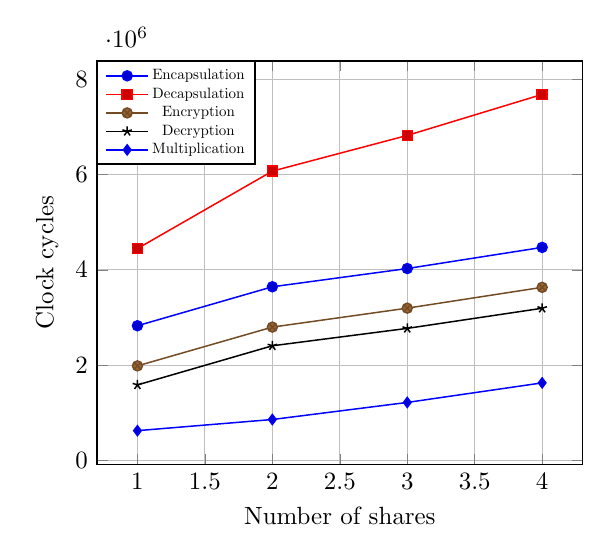
\begin{tikzpicture}[scale=0.9]
            \pgfplotsset{every axis/.append style={semithick}, legend style={at={(0,1)},anchor=north west, nodes={scale=0.6, transform shape}}}
    
        \begin{axis}[
            xlabel=Number of shares,ylabel=Clock cycles, grid=major,     x tick label style={
                /pgf/number format/.cd,
                precision=1,
            }]
    
        \addplot coordinates{
            (1, 2826067.47)
            (2, 3643555.40)
            (3, 4026514.86)
            (4, 4470225.81)
    
        };
        \addlegendentry{Encapsulation}
    
        \addplot coordinates{
            (1, 4445614.60)
            (2, 6070401.90)
            (3, 6819468.72)
            (4, 7680073.11)
    
        };
        \addlegendentry{Decapsulation}
    
        \addplot coordinates{
            (1, 1983894.79)
            (2, 2797433.27)
            (3, 3195107.26)
            (4, 3632298.13)
    
        };
        \addlegendentry{Encryption}
    
        \addplot coordinates{
            (1, 1584503.47)
            (2, 2405541.52)
            (3, 2770976.91)
            (4, 3193077.76)
    
        };
        \addlegendentry{Decryption}
    
        \addplot coordinates{
            (1, 624965.27)
            (2, 858842.66)
            (3, 1216993.20)
            (4, 1627512.25)
    
        };
        \addlegendentry{Multiplication}
        \end{axis}%
    \end{tikzpicture}%
    \end{figure}
\end{frame}

\begin{frame}{Execution Time}
    \begin{block}{Execution time (milliseconds)}
        \begin{table}
            \begin{tabular}{llllll}
                \# & encaps & decaps & enc & dec & mul \\ \hline
                1 & 201.86 & 317.54 & 141.71 & 113.18 & 44.64 \\
                2 & 260.25 & 433.60 & 199.82 & 171.82 & 61.35 \\
                3 & 287.61 & 487.10 & 228.22 & 197.93 & 86.93 \\
                4 & 319.30 & 548.58 & 259.45 & 228.08 & 116.25             
            \end{tabular}
        \end{table}
    \end{block}
    \begin{block}{Percentual performance decrease}
        \begin{table}
            \begin{tabular}{llllll}
                \# & encaps & decaps & enc & dec & mul \\ \hline
                2 & 28.92 & 36.55 & 41.00 & 51.81 & 37.42 \\
                3 & 42.48 & 53.40 & 61.05 & 74.88 & 94.73 \\
                4 & 58.18 & 72.76 & 83.09 & 101.51 & 160.41
            \end{tabular}
        \end{table}
    \end{block}
\end{frame}

\begin{frame}{Constant-time execution}
    \begin{block}{Welch's t-test}
        Given two statistical populations $X_1$ and $X_2$ of $N_1$ and $N_2$ samples respectively:
        \begin{equation*}
            t = \frac{\bar{X_1} - \bar{X_2}}{\sqrt{\frac{s_{X_1}^2}{N_1} + \frac{s_{X_2}^2}{N_2}}}
        \end{equation*}\\
    Can be used to verify that the means of the distributions are equal (null hypothesis).\\
    Setting the confidence to 99.999\%, we accept $H_0$ for $|t| \leq 4.5$
    \end{block}
\end{frame}

\begin{frame}{Constant-time execution}
    \begin{block}{Test Vector Leakage Assessment}
        Based on the Welch's t-test, defines the two groups as:
        \begin{itemize}
            \item Random: use different inputs for each computation
            \item Fixed: use the same inputs for all computations
        \end{itemize}
        In case of random data (\textit{e.g.} masks), these are always generated randomly.
    \end{block}
\end{frame}

\begin{frame}{Constant-time execution}
    \begin{block}{Welch's t}
        \begin{table}
            \begin{tabular}{llllll}
                \# & encaps & decaps & enc & dec & mul \\ \hline
                1 & 0.93666 & 4.56649 & 25.66178 & 10.26449 & 30.09420 \\
                2 & 6.00482 & 3.35650 & 4.62100 & 5.96089 & 4.96460 \\
                3 & 0.28901 & 1.69393 & 1.59911 & 5.88290 & 3.50812 \\
                4 & 0.12693 & NA\footnote{Not enough memory} & 3.30161 & 4.01299 & 0.21834
            \end{tabular}
        \end{table}        
    \end{block}
\end{frame}


\begin{frame}[allowframebreaks]
    \frametitle{References}
    \bibliographystyle{amsalpha}
    \bibliography{refs.bib}
\end{frame}

%\bibliography{refs.bib}
\end{document}
